\documentclass[12pt]{article}
 
\usepackage[margin=1in]{geometry}
\usepackage{amsmath,amsthm,amssymb}
\usepackage{mathtools}
\DeclarePairedDelimiter{\ceil}{\lceil}{\rceil}
%\usepackage{mathptmx}
\usepackage{accents}
\usepackage{comment}
\usepackage{graphicx}
\usepackage{IEEEtrantools}
 \usepackage{float}
 
\newcommand{\N}{\mathbb{N}}
\newcommand{\Z}{\mathbb{Z}}
\newcommand{\R}{\mathbb{R}}
\newcommand{\Q}{\mathbb{Q}}
\newcommand*\conj[1]{\bar{#1}}
\newcommand*\mean[1]{\bar{#1}}
\newcommand\widebar[1]{\mathop{\overline{#1}}}


\newcommand{\cc}{{\mathbb C}}
\newcommand{\rr}{{\mathbb R}}
\newcommand{\qq}{{\mathbb Q}}
\newcommand{\nn}{\mathbb N}
\newcommand{\zz}{\mathbb Z}
\newcommand{\aaa}{{\mathcal A}}
\newcommand{\bbb}{{\mathcal B}}
\newcommand{\rrr}{{\mathcal R}}
\newcommand{\fff}{{\mathcal F}}
\newcommand{\ppp}{{\mathcal P}}
\newcommand{\eps}{\varepsilon}
\newcommand{\vv}{{\mathbf v}}
\newcommand{\ww}{{\mathbf w}}
\newcommand{\xx}{{\mathbf x}}
\newcommand{\ds}{\displaystyle}
\newcommand{\Om}{\Omega}
\newcommand{\dd}{\mathop{}\,\mathrm{d}}
\newcommand{\ud}{\, \mathrm{d}}
\newcommand{\seq}[1]{\left\{#1\right\}_{n=1}^\infty}
\newcommand{\isp}[1]{\quad\text{#1}\quad}
\newcommand*\diff{\mathop{}\!\mathrm{d}}

\DeclareMathOperator{\imag}{Im}
\DeclareMathOperator{\re}{Re}
\DeclareMathOperator{\diam}{diam}
\DeclareMathOperator{\Tr}{Tr}
\DeclareMathOperator{\cis}{cis}

\def\upint{\mathchoice%
    {\mkern13mu\overline{\vphantom{\intop}\mkern7mu}\mkern-20mu}%
    {\mkern7mu\overline{\vphantom{\intop}\mkern7mu}\mkern-14mu}%
    {\mkern7mu\overline{\vphantom{\intop}\mkern7mu}\mkern-14mu}%
    {\mkern7mu\overline{\vphantom{\intop}\mkern7mu}\mkern-14mu}%
  \int}
\def\lowint{\mkern3mu\underline{\vphantom{\intop}\mkern7mu}\mkern-10mu\int}




\newenvironment{theorem}[2][Theorem]{\begin{trivlist}
\item[\hskip \labelsep {\bfseries #1}\hskip \labelsep {\bfseries #2.}]}{\end{trivlist}}
\newenvironment{lemma}[2][Lemma]{\begin{trivlist}
\item[\hskip \labelsep {\bfseries #1}\hskip \labelsep {\bfseries #2.}]}{\end{trivlist}}
\newenvironment{exercise}[2][Exercise]{\begin{trivlist}
\item[\hskip \labelsep {\bfseries #1}\hskip \labelsep {\bfseries #2.}]}{\end{trivlist}}
\newenvironment{problem}[2][Problem]{\begin{trivlist}
\item[\hskip \labelsep {\bfseries #1}\hskip \labelsep {\bfseries #2.}]}{\end{trivlist}}
\newenvironment{question}[2][Question]{\begin{trivlist}
\item[\hskip \labelsep {\bfseries #1}\hskip \labelsep {\bfseries #2.}]}{\end{trivlist}}
\newenvironment{corollary}[2][Corollary]{\begin{trivlist}
\item[\hskip \labelsep {\bfseries #1}\hskip \labelsep {\bfseries #2.}]}{\end{trivlist}}

\newenvironment{solution}{\begin{proof}[Solution]}{\end{proof}}
 
\begin{document}
 
% --------------------------------------------------------------
%                         Start here
% --------------------------------------------------------------
\title{Math 132A Homework 5}
\author{Ethan Martirosyan}
\date{\today}
\maketitle
\hbadness=99999
\hfuzz=50pt
\section*{Problem 1}
\subsection*{Part A}
Before we compute the gradient and Hessian of $f$, we first must compute
\[
f(x) = \frac{1}{2}x^T Q x - bx
\] We first write
\[
Qx = \begin{pmatrix}
q_{11} & q_{12} & \cdots & q_{1n}\\
q_{21} & q_{22} & \cdots & q_{2n}\\
\vdots & \vdots & \ddots & \vdots\\
q_{n1} & q_{n2} & \cdots & q_{nn}
\end{pmatrix}
\begin{pmatrix}
x_1 \\ x_2 \\ \vdots \\ x_n
\end{pmatrix}
=
\begin{pmatrix}
\sum_{j=1}^n q_{1j}x_j\\
\sum_{j=1}^n q_{2j}x_j\\
\vdots\\
\sum_{j=1}^n q_{nj}x_j
\end{pmatrix}
\] Next we compute
\[
x^TQx =
\begin{pmatrix}
x_1 & x_2 & \cdots & x_n
\end{pmatrix}
\begin{pmatrix}
\sum_{j=1}^n q_{1j}x_j\\
\sum_{j=1}^n q_{2j}x_j\\
\vdots\\
\sum_{j=1}^n q_{nj}x_j
\end{pmatrix} = \sum_{i=1}^n \sum_{j=1}^n q_{ij} x_i x_j
\] Now, we wish to take the partial derivative with respect to $x_k$ for an arbitrary $k \in \{1,\ldots,n\}$. First, we rewrite $x^TQx$ as follows:
\[
\sum_{i=1}^n \sum_{j=1}^n q_{ij} x_i x_j = q_{kk}x_k^2 + \sum\limits_{\substack{j=1 \\ j \neq k }}^n q_{kj} x_{k} x_{j} + \sum\limits_{\substack{i=1 \\ i\neq k }}^n q_{ik}x_{i}x_{k} + \sum\limits_{\substack{j\neq k \\ i \neq k }} q_{ij}x_{i}x_{j}
\] Now, we note that
\[
\frac{\partial}{\partial x_k} q_{kk} x_k^2 = 2q_{kk} x_k
\] Next, we find that
\[
\frac{\partial}{\partial x_{k}}  \sum\limits_{\substack{j=1 \\ j \neq k }}^n q_{kj} x_{k} x_{j} = \sum\limits_{\substack{j=1 \\ j \neq k }}^n q_{kj} x_j
\] and
\[
\frac{\partial}{\partial x_{k}} \sum\limits_{\substack{i=1 \\ i\neq k }}^n q_{ik}x_{i}x_{k} = \sum\limits_{\substack{i=1 \\ i\neq k }}^n q_{ik}x_{i} 
\] But we know that $Q$ is symmetric, so we obtain
\[
\sum\limits_{\substack{i=1 \\ i\neq k }}^n q_{ik}x_{i}  = \sum\limits_{\substack{i=1 \\ i\neq k }}^n q_{ki}x_{i}
\] Finally, we note
\[
\frac{\partial}{\partial x_k}  \sum\limits_{\substack{j\neq k \\ i \neq k }} q_{ij}x_{i}x_{j} = 0
\] Putting it all together, we obtain
\[
\frac{\partial}{\partial x_k} \sum_{i=1}^n \sum_{j=1}^n q_{ij} x_i x_j  =  2q_{kk} x_k +  \sum\limits_{\substack{j=1 \\ j \neq k }}^n q_{kj} x_j +  \sum\limits_{\substack{i=1 \\ i\neq k }}^n q_{ki}x_{i}  = 2q_{kk}x_k + 2  \sum\limits_{\substack{i=1 \\ i\neq k }}^n q_{ki}x_{i} = 2 \sum_{i=1}^n q_{ki} x_i
\] Remembering the factor of $1/2$, we obtain
\[
\frac{\partial}{\partial x_k} \frac{1}{2} \sum_{i=1}^n \sum_{j=1}^n q_{ij} x_i x_j = \sum_{i=1}^n q_{ki} x_i
\] Next, we compute 
\[
b^T x =
\begin{pmatrix}
b_1 & b_2 & \cdots & b_n
\end{pmatrix} 
\begin{pmatrix}
x_1 \\ x_2 \\ \vdots \\ x_n
\end{pmatrix} = \sum_{i=1}^n b_i x_i
\] In this case, taking the partial derivative with respect to $x_k$ yields
\[
\frac{\partial}{\partial x_k} \sum_{i=1}^n b_i x_i = b_k
\] Thus, we find that
\[
\frac{\partial}{\partial x_k} f(x) =  \sum_{i=1}^n q_{ki} x_i - b_k
\] So, in particular, we have
\[
\nabla f(x) = \begin{pmatrix}
\sum_{i=1}^n q_{1i} x_i - b_1
\\
\vdots
\\
\sum_{i=1}^n q_{ni} x_i - b_n
\end{pmatrix}
\] But we also have
\[
Qx - b = \begin{pmatrix}
\sum_{i=1}^n q_{1i}x_i\\
\vdots\\
\sum_{i=1}^n q_{ni}x_i
\end{pmatrix} 
- \begin{pmatrix}
b_1\\
\vdots\\
b_n
\end{pmatrix} = \begin{pmatrix}
\sum_{i=1}^n q_{1i} x_i - b_1
\\
\vdots
\\
\sum_{i=1}^n q_{ni} x_i - b_n
\end{pmatrix}
\] so we obtain
\[
\nabla f(x) = Qx - b
\] To find the Hessian, we first use the fact that for an arbitrary $k \in \{1,\ldots,n\}$, we have
\[
\frac{\partial}{\partial x_k} f(x) =  \sum_{i=1}^n q_{ki} x_i - b_k
\] Now, let us take the partial derivative of this expression with respect to $x_l$ for an arbitrary $l \in \{1,\ldots,n\}$. We obtain
\[
\frac{\partial^2}{\partial x_l \partial x_k} f(x) = \frac{\partial}{\partial x_l} \sum_{i=1}^n q_{ki} x_i - b_k = q_{kl}
\] Now, we know that the entry in row $l$ and column $k$ of the Hessian is 
\[
\frac{\partial^2}{\partial x_l \partial x_k} f(x) = q_{kl} = q_{lk} 
\] So we find that 
\[
\nabla^2 f(x) = \begin{pmatrix}
q_{11} & \cdots & q_{1n}\\
\vdots & \ddots & \vdots\\
q_{n1} & \cdots & q_{nn}
\end{pmatrix} = Q
\]
\newpage
\subsection*{Part B}
First, we compute
\begin{align*}
f(x) = \frac{1}{2}x^TQx - b^T x = \frac{1}{2}\begin{bmatrix}
x_1 & x_2
\end{bmatrix}
\begin{bmatrix}
3 & -1\\
-1 & 1
\end{bmatrix}
\begin{bmatrix}
x_1\\
x_2
\end{bmatrix}
- \begin{bmatrix}
2 & 1
\end{bmatrix}
\begin{bmatrix}
x_1\\
x_2
\end{bmatrix}
= \frac{3}{2} x_1^2 - x_1x_2 + \frac{1}{2}x_2^2 - 2x_1 - x_2
\end{align*} Now, we compute the gradient 
\[
\nabla f(x) = 
\begin{bmatrix}
3x_1 - x_2 - 2\\
-x_1 + x_2 - 1
\end{bmatrix}
\] Now, we find
\[
\nabla f(x^{(0)}) = \nabla f(1,1.5) = \begin{bmatrix}
3(1) - 1.5 - 2\\
-1 + 1.5 - 1
\end{bmatrix} = 
\begin{bmatrix}
-0.5\\
-0.5
\end{bmatrix}
\] Now, we wish to take
\[
x^{(1)} = x^{(0)} - \alpha \nabla f(x^{(0)}) 
\] for optimal $\alpha$. But from class, we know that 
\[
\alpha_0 = \frac{(\nabla f(x^{(0)}))^T \nabla f(x^{(0)})}{(\nabla f(x^{(0)}))^TQ \nabla f(x^{(0)})}
\] First, we compute 
\[
(\nabla f(x^{(0)}))^T \nabla f(x^{(0)}) = \begin{bmatrix}
-0.5 & -0.5
\end{bmatrix}
\begin{bmatrix}
-0.5 \\
-0.5
\end{bmatrix} = 0.25+0.25 = 0.5
\] Next, we compute 
\[
(\nabla f(x^{(0)}))^TQ \nabla f(x^{(0)}) =
 \begin{bmatrix}
-0.5 & -0.5
\end{bmatrix}
\begin{bmatrix}
3 & -1\\
-1 & 1
\end{bmatrix}
\begin{bmatrix}
-0.5 \\
-0.5
\end{bmatrix}
= 0.5
\] So we obtain
\[
\alpha_0 = \frac{(\nabla f(x^{(0)}))^T \nabla f(x^{(0)})}{(\nabla f(x^{(0)}))^TQ \nabla f(x^{(0)})} = \frac{0.5}{0.5} = 1
\] which gives us
\[
x^{(1)} = x^{(0)} - \alpha \nabla f(x^{(0)})  = \begin{bmatrix}
1\\
1.5
\end{bmatrix} - 1 \begin{bmatrix}
-0.5 \\ -0.5
\end{bmatrix} =
\begin{bmatrix}
1.5\\
2
\end{bmatrix}
\] Now, we compute
\[
\nabla f(x^{(1)}) = \nabla f(1.5,2) = \begin{bmatrix}
3(1.5) - 2 - 2\\
-1.5 + 2 - 1
\end{bmatrix} = 
\begin{bmatrix}
0.5 \\
-0.5
\end{bmatrix}
\] This time, we find
\[
\alpha_1 = \frac{(\nabla f(x^{(1)}))^T \nabla f(x^{(1)})}{(\nabla f(x^{(1)}))^TQ \nabla f(x^{(1)})} 
\] We compute
\[
(\nabla f(x^{(1)}))^T \nabla f(x^{(1)}) = \begin{bmatrix}
0.5 & -0.5
\end{bmatrix} \begin{bmatrix}
0.5 \\
-0.5
\end{bmatrix} = 0.25 + 0.25 = 0.5
\] and
\[
(\nabla f(x^{(1)}))^TQ \nabla f(x^{(1)}) =
\begin{bmatrix}
0.5 & -0.5
\end{bmatrix}
\begin{bmatrix}
3 & -1\\
-1 & 1
\end{bmatrix}
 \begin{bmatrix}
0.5 \\
-0.5
\end{bmatrix} = 1.5
\] So we find that
\[
\alpha_1 = \frac{(\nabla f(x^{(1)}))^T \nabla f(x^{(1)})}{(\nabla f(x^{(1)}))^TQ \nabla f(x^{(1)})}  = \frac{0.5}{1.5} = \frac{1}{3}
\] and we obtain
\[
x^{(2)} = x^{(1)} - \alpha_1 \nabla f(x^{(1)}) = \begin{bmatrix}
1.5\\
2
\end{bmatrix} - \frac{1}{3} \begin{bmatrix}
0.5 \\
-0.5
\end{bmatrix} = \begin{bmatrix}
4/3\\
13/6
\end{bmatrix}
\] Finally, we compute
\[
\nabla f(x^{(2)}) = \begin{bmatrix}
3(4/3) - 13/6 - 2\\
-4/3 + 13/6 - 1
\end{bmatrix}
=\begin{bmatrix}
-1/6\\
-1/6
\end{bmatrix}
\] Again, we have 
\[
\alpha_2 = \frac{(\nabla f(x^{(2)}))^T \nabla f(x^{(2)})}{(\nabla f(x^{(2)}))^TQ \nabla f(x^{(2)})}
\] We note that
\[
(\nabla f(x^{(2)}))^T \nabla f(x^{(2)}) = \begin{bmatrix}
-1/6 & -1/6
\end{bmatrix} \begin{bmatrix}
-1/6\\
-1/6
\end{bmatrix} = \frac{1}{36} + \frac{1}{36} = \frac{1}{18}
\] and
\[
(\nabla f(x^{(2)}))^TQ \nabla f(x^{(2)}) = 
\begin{bmatrix}
-1/6 & -1/6
\end{bmatrix} 
\begin{bmatrix}
3 & -1\\
-1 & 1
\end{bmatrix}
\begin{bmatrix}
-1/6\\
-1/6
\end{bmatrix} = \frac{1}{18}
\] So we find that
\[
\alpha_2 = \frac{(\nabla f(x^{(2)}))^T \nabla f(x^{(2)})}{(\nabla f(x^{(2)}))^TQ \nabla f(x^{(2)})} = \frac{1/18}{1/18} = 1
\] Finally, we obtain
\[
x^{(3)} = x^{(2)} - \alpha_2 \nabla f(x^{(2)}) = 
\begin{bmatrix}
4/3\\
13/6
\end{bmatrix} - 1\begin{bmatrix}
-1/6\\
-1/6
\end{bmatrix} = 
\begin{bmatrix}
3/2\\
7/3
\end{bmatrix}
\]




\newpage
\section*{Problem 2}
First, we compute the gradient as follows:
\[
\nabla f(x) = \begin{bmatrix}
x_2e^{x_1x_2} + 2x_1 x_2^2\\
x_1e^{x_1x_2} + 2x_1^2 x_2
\end{bmatrix}
\] Now, we plug in the point $x^{(0)}$:
\[
\nabla f(x^{(0)}) = \nabla f(0,-2) =
 \begin{bmatrix}
-2e^{0\cdot-2} + 2(0)(-2)^2\\
0e^{0 \cdot - 2} + 2(0)^2 (-2)
\end{bmatrix} = \begin{bmatrix}
-2\\
0
\end{bmatrix}
\] Now, we wish to find an $\alpha$ that minimizes the following expression:
\[
f(x^{(0)}-\alpha \nabla f(x^{(0)})) = f(2\alpha, -2) = e^{-4\alpha} + 16\alpha^2
\] According to Wolfram Alpha, we find that
\[
\alpha_0 \approx 0.087933427812299
\] Now, we compute
\[
x^{(1)} = x^{(0)} - \alpha_0 \nabla f(x^{(0)}) = 
 \begin{bmatrix}
0\\
-2
\end{bmatrix} - \alpha_0 \begin{bmatrix}
-2\\
0
\end{bmatrix} =
\begin{bmatrix}
0.175866855624598\\
-2
\end{bmatrix}
\] Now, we compute
\[
\nabla f(x^{(1)}) =  \begin{bmatrix}
0\\
0
\end{bmatrix}
\] I obtained this result from Matlab. We wish to find $\alpha$ that minimizes
\[
f(x^{(1)} - \alpha \nabla f(x^{(1)}))
\] Well, we can just take $\alpha_1 = 0$. So we have
\[
x^{(2)} = x^{(1)} - \alpha_1   \nabla f(x^{(1)}) = \begin{bmatrix}
0.176\\
-2
\end{bmatrix} - 0 \begin{bmatrix}
0\\
0
\end{bmatrix} = 
 \begin{bmatrix}
0.176\\
2
\end{bmatrix} 
\] For the third iteration, we will just have
\[
x^{(3)} = x^{(2)}
\]

\newpage
\section*{Problem 3}
\subsection*{Part A}
First, we note that
\[
f(x_1,x_2) = 100(x_2-x_1^2)^2 + (1-x_1)^2 \geq 0
\] for all $x_1$ and $x_2$. To find the minimizers, we may set
\[
100(x_2-x_1^2)^2 + (1-x_1)^2 = 0
\] This can only be true if $1-x_1 = 0$ and $x_2 - x_1^2 = 0$. The first equation tells us that $x_1 = 1$ and the second equation tells us that $x_2 = 1$. Thus, we find that $(1,1)$ is the unique global minimizer.
\newpage
\subsection*{Part B}
First, we compute the gradient of $f$ as follows:
\[
\nabla f(x) =
\begin{bmatrix}
 -400 x_1 (x_2 - x_1^2) - 2(1-x_1)\\
 200(x_2 - x_1^2)
\end{bmatrix}
\] Next, we compute the Hessian:
\[
\nabla^2 f(x) = 
\begin{bmatrix}
-400 x_2 + 1200 x_1^2 + 2 & -400x_1\\
-400x_1 & 200
\end{bmatrix}
\] Now, we note that
\[
x^{(1)} = x^{(0)} - [\nabla^2 f(x^{(0)})]^{-1} \nabla f(x^{(0)}) 
\] First, we compute 
\[
 \nabla f(x^{(0)})  = \nabla f(0,0) = \begin{bmatrix}
 -400 (0) (0 - 0^2) - 2(1-0)\\
 200(0 - 0^2)
\end{bmatrix}
= \begin{bmatrix}
-2\\
0
\end{bmatrix}
\] and 
\[
\nabla^2 f(x^{(0)}) = \nabla^2 f(0,0) = \begin{bmatrix}
2 & 0\\
0 & 200
\end{bmatrix}
\] so that
\[
[\nabla^2 f(x^{(0)})]^{-1} = \begin{bmatrix}
1/2 & 0\\
0 & 1/200
\end{bmatrix}
\] which gives us 
\[
[\nabla^2 f(x^{(0)})]^{-1} \nabla f(x^{(0)})  = \begin{bmatrix} -1 \\ 0
\end{bmatrix}
\] so we finally obtain
\[
x^{(1)} = x^{(0)} - [\nabla^2 f(x^{(0)})]^{-1} \nabla f(x^{(0)}) = \begin{bmatrix} 0 \\ 0
\end{bmatrix} - \begin{bmatrix} -1 \\ 0 \end{bmatrix} = \begin{bmatrix} 1 \\ 0 \end{bmatrix}
\] Next, we compute
\[
\nabla f(x^{(1)}) = \nabla f(1,0) = 
\begin{bmatrix}
 -400\cdot 1 \cdot (0 - 1^2) - 2(1-1)\\
 200(0 - 1^2)
\end{bmatrix}
= \begin{bmatrix}
400\\
-200
\end{bmatrix}
\] and
\[
\nabla^2 f(x^{(1)}) = \nabla^2 f(1,0) = \begin{bmatrix}
-400 \cdot 0 + 1200 \cdot 1^2 + 2 & -400\cdot 1\\
-400\cdot 1 & 200
\end{bmatrix} = 
\begin{bmatrix}
1202 & -400\\
-400 & 200
\end{bmatrix}
\] Then, we compute
\[
[\nabla^2 f(x^{(1)})]^{-1} = \frac{1}{80400} \begin{bmatrix}
200 & 400\\
400 & 1202
\end{bmatrix}
\] From this, we obtain
\[
[\nabla^2 f(x^{(1)})]^{-1} \nabla f(x^{(1)}) = \frac{1}{80400} \begin{bmatrix}
200 & 400\\
400 & 1202
\end{bmatrix} \begin{bmatrix}
400\\
-200
\end{bmatrix} = \begin{bmatrix}
0 \\ -1
\end{bmatrix}
\] Finally, we find that
\[
x^{(2)} = x^{(1)} - [\nabla^2 f(x^{(1)})]^{-1} \nabla f(x^{(1)}) = \begin{bmatrix} 1\\ 0 \end{bmatrix} - \begin{bmatrix} 0 \\ -1 \end{bmatrix} = \begin{bmatrix} 1 \\ 1
\end{bmatrix}
\]
\newpage
\subsection*{Part C}
Now, we apply the steepest descent method with $\alpha = 0.05$. First, we compute
\[
 x^{(1)} = x^{(0)} - \alpha \nabla f(x^{(0)}) = 
 \begin{bmatrix}
 0 \\
 0
 \end{bmatrix} - 0.05 \begin{bmatrix}
 -2 \\ 0
 \end{bmatrix} = 
\begin{bmatrix}
0.1 \\
0
\end{bmatrix}
\]
 Next, we compute
\[
\nabla f(x^{(1)}) =  \nabla f(0.1,0) = 
\begin{bmatrix}
-400(0.1)(0-0.1^2) - 2(1-0.1)\\
200(0 - 0.1^2)
\end{bmatrix}
=
\begin{bmatrix}
-1.4\\
-2
\end{bmatrix}
\] Thus, we find that
\[
x^{(2)} = x^{(1)} - \alpha \nabla f(x^{(1)}) = \begin{bmatrix} 0.1\\ 0
\end{bmatrix} - 0.05 \begin{bmatrix} -1.4 \\ - 2
\end{bmatrix} = \begin{bmatrix} 0.17\\ 0.1
\end{bmatrix}
\]
\newpage
\section*{Problem 4}
First, we compute 
\[
\nabla f(x^{(0)}) = Qx^{(0)} - b =
\begin{bmatrix}
4 & 2\\
2 & 2
\end{bmatrix}
\begin{bmatrix}
0\\
0
\end{bmatrix} -
\begin{bmatrix}
-1\\
1
\end{bmatrix}=
\begin{bmatrix}
1\\
-1
\end{bmatrix}
\] and
\[
p^{(0)} =  B_0^{-1} \nabla f(x^{(0)}) = I^{-1} \nabla f(x^{(0)}) = \begin{bmatrix}
1\\
-1
\end{bmatrix} 
\] We wish to find an $\alpha$ that minimizes the expression
\[
f(x^{(0)} - \alpha p^{(0)})
\]  In order to do this effectively, we set
\begin{align*}
g(\alpha) & = f(x^{(0)} - \alpha p^{(0)}) = \frac{1}{2} \big(x^{(0)} - \alpha p^{(0)}\big)^T Q (x^{(0)} - \alpha p^{(0)}) - b^T(x^{(0)} - \alpha p^{(0)})\\
& = \frac{1}{2}(x^{(0)})^T Q x^{(0)} - \alpha (x^{(0)})^T Q p^{(0)} + \frac{1}{2}\alpha^2 (p^{(0)})^T Q p^{(0)} - b^T x^{(0)} + \alpha b^T p^{(0)}
\end{align*}
Now, we want to minimize this expression, so we take
\begin{align*}
g^\prime(\alpha) &= \alpha (p^{(0)})^T Q p^{(0)} - (x^{(0)})^T Q p^{(0)} + b^T p^{(0)} = \alpha (p^{(0)})^T Q p^{(0)} - (Qx^{(0)} - b)^T p^{(0)}\\
&=  \alpha (p^{(0)})^T Q p^{(0)} - (\nabla f(x^{(0)}))^T p^{(0)} = 0
\end{align*} Solving for $\alpha$ gives us
\[
\alpha = \frac{(\nabla f(x^{(0)}))^Tp^{(0)}}{(p^{(0)})^TQp^{(0)}}
\]

Now, we compute
\[
\alpha_0 = \frac{(\nabla f(x^{(0)}))^Tp^{(0)}}{(p^{(0)})^TQp^{(0)}}
\] Notice that
\[
(\nabla f(x^{(0)}))^Tp^{(0)} = \begin{bmatrix} 1 & -1
\end{bmatrix} \begin{bmatrix} 1 \\ -1
\end{bmatrix} = 2
\] and
\[
(p^{(0)})^TQp^{(0)} = \begin{bmatrix} 1 & -1
\end{bmatrix} \begin{bmatrix}
4 & 2\\
2 & 2
\end{bmatrix} \begin{bmatrix} 1 \\ -1
\end{bmatrix}  = 2
\] so that
\[
\alpha_0 = \frac{(\nabla f(x^{(0)}))^Tp^{(0)}}{(p^{(0)})^TQp^{(0)}} = \frac{2}{2} = 1
\] So we obtain
\[
x^{(1)} = x^{(0)} - \alpha_0 p^{(0)} =
\begin{bmatrix}
0\\
0
\end{bmatrix} - 1 \begin{bmatrix}
1\\
-1
\end{bmatrix} = \begin{bmatrix}
-1\\
1
\end{bmatrix}
\] Now we compute 
\[
\nabla f(x^{(1)}) = Qx^{(1)} - b = \begin{bmatrix}
4 & 2\\
2 & 2
\end{bmatrix} \begin{bmatrix}
-1\\
1
\end{bmatrix} - \begin{bmatrix}
-1\\
1
\end{bmatrix} = \begin{bmatrix}
-1 \\ -1
\end{bmatrix}
\]Now, we find
\[
s_0 = x^{(1)} - x^{(0)} = \begin{bmatrix}
-1\\
1
\end{bmatrix}
\] And we also have
\[
y_0 = \nabla f(x^{(1)}) - \nabla f(x^{(0)}) = \begin{bmatrix}
-1 \\ -1
\end{bmatrix} - \begin{bmatrix}
1\\
-1
\end{bmatrix} = 
\begin{bmatrix}
-2\\
0
\end{bmatrix}
\] Now, we wish to compute
\[
B_{1} = \frac{(y_0 - B_0 s_0)(y_0 - B_0 s_0)^T}{(y_0 - B_0 s_0)^Ts_0}
\] First, we should probably check that the denominator is nonzero. So we have
\[
(y_0 - B_0 s_0)^T s_0 = 
\begin{bmatrix}
-1 & - 1
\end{bmatrix}
\begin{bmatrix}
-1\\
1
\end{bmatrix} = 0
\] Since the denominator is $0$, we can just let $B_1 = B_0 = I$.
Now, we take
\[
p^{(1)} = B_1^{-1} \nabla f(x^{(1)}) = 
\begin{bmatrix}
-1\\
-1
\end{bmatrix}
\] To find the optimal $\alpha$, we take
\[
\alpha_1 = \frac{(\nabla f(x^{(1)}))^T p^{(1)}  }{(p^{(1)})^TQ p^{(1)} }
\] Notice that
\[
(\nabla f(x^{(1)}))^T p^{(1)} =   \begin{bmatrix}
-1 & -1
\end{bmatrix}  \begin{bmatrix}
-1 \\ -1
\end{bmatrix} = 2 
\] and
\[
(p^{(1)})^TQ p^{(1)} = 
\begin{bmatrix}
-1 & -1
\end{bmatrix} \begin{bmatrix}
4 & 2\\
2 & 2
\end{bmatrix}  \begin{bmatrix}
-1 \\ -1
\end{bmatrix} = 10
\] so that
\[
\alpha_1 = \frac{2}{10} = 0.2
\] So now we take
\[
x^{(2)} = x^{(1)} - \alpha_1 p^{(1)} = \begin{bmatrix}
-1\\
1
\end{bmatrix} - 0.2 \begin{bmatrix}
-1\\
-1
\end{bmatrix} = 
\begin{bmatrix}
-0.8\\
1.2
\end{bmatrix}
\] Then, we take
\[
s_1 = x^{(2)} - x^{(1)} = \begin{bmatrix}
-0.8\\
1.2
\end{bmatrix} -  \begin{bmatrix}
-1\\
1
\end{bmatrix} =
\begin{bmatrix}
0.2\\
0.2
\end{bmatrix}
\]
Next, we compute
\[
\nabla f(x^{(2)}) = Qx^{(2)} - b = \begin{bmatrix}
4 & 2\\
2 & 2
\end{bmatrix} \begin{bmatrix}
-0.8\\
1.2
\end{bmatrix} - \begin{bmatrix}
-1\\
1
\end{bmatrix} =
\begin{bmatrix}
0.2\\
-0.2
\end{bmatrix}
\] Then, we take
\[
y_1 = \nabla f(x^{(2)}) - \nabla f(x^{(1)}) = \begin{bmatrix}
0.2\\
-0.2
\end{bmatrix} -  \begin{bmatrix}
-1 \\ -1
\end{bmatrix} = 
 \begin{bmatrix}
1.2 \\ 0.8
\end{bmatrix} 
\] Now, we compute
\[
y_1 - B_1 s_1 = y_1 - s_1 =  \begin{bmatrix}
1.2 \\ 0.8
\end{bmatrix} - \begin{bmatrix}
0.2\\
0.2
\end{bmatrix} =
\begin{bmatrix}
1\\
0.6
\end{bmatrix}
\] So we find that
\[
(y_1 - B_1 s_1)(y_1 - B_1 s_1)^T = \begin{bmatrix}
1\\
0.6
\end{bmatrix} \begin{bmatrix}
1 & 0.6
\end{bmatrix} =
\begin{bmatrix}
1 & 0.6\\
0.6 & 0.36
\end{bmatrix}
\] and
\[
(y_1 - B_1 s_1)^T s_1 = \begin{bmatrix}
1 & 0.6
\end{bmatrix}  \begin{bmatrix}
0.2\\
0.2
\end{bmatrix} = 0.32
\] So we obtain
\[
U_1 = \frac{(y_1 - B_1 s_1)(y_1 - B_1 s_1)^T}{(y_1 - B_1 s_1)^T s_1} = 
\begin{bmatrix}
3.125 & 1.875\\
1.875 & 1.125
\end{bmatrix}
\] and we take
\[
B_2 = B_1 + U_1 =\begin{bmatrix}
1 & 0\\
0 & 1
\end{bmatrix}+  \begin{bmatrix}
3.125 & 1.875\\
1.875 & 1.125
\end{bmatrix} =
 \begin{bmatrix}
4.125 & 1.875\\
1.875 & 2.125
\end{bmatrix}
\]
\newpage
\section*{Problem 5}
For the first iteration, we compute
\[
\nabla f(x^{(0)}) = Qx^{(0)} - b = 
\begin{bmatrix}
3 & -1\\
-1 & 1
\end{bmatrix}
\begin{bmatrix}
1\\
1.5
\end{bmatrix} - 
\begin{bmatrix}
2\\
1
\end{bmatrix} = 
\begin{bmatrix}
-0.5\\
-0.5
\end{bmatrix}
\] Then, we compute
\[
p^{(0)} = B_0^{-1} \nabla f(x^{(0)}) = I^{-1} \nabla f(x^{(0)}) = \nabla f(x^{(0)}) = 
\begin{bmatrix}
-0.5\\
-0.5
\end{bmatrix}
\] Now, we compute
\[
\alpha_0 = \frac{(\nabla f(x^{(0)}))^T p^{(0)}}{(p^{(0)})^T Q p^{(0)}}
\] We notice that
\[
(\nabla f(x^{(0)}))^T p^{(0)} = 
\begin{bmatrix}
-0.5 & -0.5
\end{bmatrix}
\begin{bmatrix}
-0.5\\
-0.5
\end{bmatrix}
= 0.25 + 0.25 = 0.5
\] and
\[
(p^{(0)})^T Q p^{(0)} = 
\begin{bmatrix}
-0.5 &
-0.5
\end{bmatrix} \begin{bmatrix}
3 & -1\\
-1 & 1
\end{bmatrix} \begin{bmatrix}
-0.5\\
-0.5
\end{bmatrix} = 0.5
\] Thus, we find that
\[
\alpha_0 = \frac{(\nabla f(x^{(0)}))^T p^{(0)}}{(p^{(0)})^T Q p^{(0)}} = \frac{0.5}{0.5} = 1
\] So we get
\[
x^{(1)} = x^{(0)} - \alpha_0 p^{(0)} = \begin{bmatrix}
1\\
1.5
\end{bmatrix} - 1 \begin{bmatrix}
-0.5\\
-0.5
\end{bmatrix} = \begin{bmatrix}
1.5\\
2
\end{bmatrix}
\] Now, we compute
\[
\nabla f(x^{(1)}) = Qx^{(1)} - b = \begin{bmatrix}
3 & -1\\
-1 & 1
\end{bmatrix}
\begin{bmatrix}
1.5\\
2
\end{bmatrix} - 
\begin{bmatrix}
2\\
1
\end{bmatrix} = 
\begin{bmatrix}
0.5\\
-0.5
\end{bmatrix}
\] Then, we find that
\[
s_0 = x^{(1)} - x^{(0)} =  \begin{bmatrix}
1.5\\
2
\end{bmatrix}  - \begin{bmatrix}
1\\
1.5
\end{bmatrix} =
 \begin{bmatrix}
0.5\\
0.5
\end{bmatrix}
 \]
 and
\[
y_0 = \nabla f(x^{(1)}) - \nabla f(x^{(0)}) = 
\begin{bmatrix}
0.5\\
-0.5
\end{bmatrix} - \begin{bmatrix}
-0.5\\
-0.5
\end{bmatrix} = 
\begin{bmatrix}
1\\
0
\end{bmatrix}
\] Now, we find that
\[
B_1 = B_0 - \frac{B_0 s_0 (s_0)^T B_0}{(s_0)^T B_0 s_0} + \frac{y_0 (y_0)^T}{(y_0)^T s_0}
\] First, we compute
\[
B_0 s_0 (s_0)^T B_0 = 
\begin{bmatrix}
1 & 0\\
0 & 1 
\end{bmatrix}
\begin{bmatrix}
0.5\\
0.5 
\end{bmatrix}
\begin{bmatrix}
0.5 & 0.5 
\end{bmatrix}
\begin{bmatrix}
1 & 0\\
0 & 1 
\end{bmatrix} =
\begin{bmatrix}
0.25 & 0.25\\
0.25 & 0.25 
\end{bmatrix} 
\] Next, we compute
\[
(s_0)^T B_0 s_0 =
\begin{bmatrix}
0.5 & 0.5 
\end{bmatrix}
\begin{bmatrix}
1 & 0\\
0 & 1 
\end{bmatrix}
\begin{bmatrix}
0.5\\
0.5 
\end{bmatrix} = 0.5
\] And then we compute
\[
y_0(y_0)^T = \begin{bmatrix}
1\\
0
\end{bmatrix} 
\begin{bmatrix}
1 & 0
\end{bmatrix} 
=
\begin{bmatrix}
1 & 0\\
0 & 0
\end{bmatrix}
\]
and 
\[
(y_0)^T s_0 = \begin{bmatrix}
1 & 0
\end{bmatrix} \begin{bmatrix}
0.5 \\ 0.5
\end{bmatrix} = 0.5
\] All in all, we get
\[
B_1 = \begin{bmatrix}
1 & 0\\
0 & 1
\end{bmatrix} - \frac{1}{0.5} 
\begin{bmatrix}
0.25 & 0.25\\
0.25 & 0.25
\end{bmatrix} +
\frac{1}{0.5} \begin{bmatrix}
1 & 0\\
0 & 0
\end{bmatrix} = 
\begin{bmatrix}
2.5 & -0.5\\
-0.5 & 0.5
\end{bmatrix}
\] Next, we take
\[
p^{(1)} = B_1^{-1} \nabla f(x^{(1)}) = 
\begin{bmatrix}
0.5 & 0.5\\
0.5 & 2.5
\end{bmatrix}
\begin{bmatrix}
0.5 \\
-0.5
\end{bmatrix} =
\begin{bmatrix}
0\\
-1
\end{bmatrix}
\] Next, we wish to compute
\[
\alpha_1 = \frac{\nabla f(x^{(1)})^T p^{(1)}  }{(p^{(1)} )^T Q p^{(1)} }
\] Notice that
\[
\nabla f(x^{(1)})^T p^{(1)} =
\begin{bmatrix}
0.5 & -0.5
\end{bmatrix}
\begin{bmatrix}
0\\
-1
\end{bmatrix} = 0.5
\] and
\[
(p^{(1)} )^T Q p^{(1)}  = 
\begin{bmatrix}
0& -1
\end{bmatrix}
\begin{bmatrix}
3 & -1\\
-1 & 1
\end{bmatrix}
\begin{bmatrix}
0\\
-1
\end{bmatrix} = 1
\] So we find that
\[
\alpha_1 = \frac{\nabla f(x^{(1)})^T p^{(1)}  }{(p^{(1)} )^T Q p^{(1)} } = \frac{0.5}{1} = 0.5
\] With this, we obtain
\[
x^{(2)} = x^{(1)} - \alpha_1 p^{(1)} = 
\begin{bmatrix}
1.5\\
2
\end{bmatrix} - 1\begin{bmatrix}
0\\
-0.5
\end{bmatrix} =
\begin{bmatrix}
1.5\\
2.5
\end{bmatrix} 
\] We also find
\[
\nabla f(x^{(2)}) = Q x^{(2)} - b = \begin{bmatrix}
3 & -1\\
-1 & 1
\end{bmatrix}
\begin{bmatrix}
1.5\\
2.5
\end{bmatrix} - 
\begin{bmatrix}
2\\
1
\end{bmatrix} =
\begin{bmatrix}
0\\
0
\end{bmatrix}
\] Now, we compute
\[
s_1 = x^{(2)} - x^{(1)} = \begin{bmatrix}
1.5\\
2.5
\end{bmatrix} - \begin{bmatrix}
1.5\\
2
\end{bmatrix} =
\begin{bmatrix}
0\\
0.5
\end{bmatrix} 
\] and
\[
y_1 = \nabla f(x^{(2)}) - \nabla f(x^{(1)}) = 
\begin{bmatrix}
0\\
0
\end{bmatrix} - 
\begin{bmatrix}
0.5\\
-0.5
\end{bmatrix} =
\begin{bmatrix}
-0.5\\
0.5
\end{bmatrix}
\] This time, we find that
\[
B_2 = B_1 - \frac{B_1 s_1 (s_1)^T B_1}{(s_1)^T B_1 s_1} + \frac{y_1 (y_1)^T}{(y_1)^T s_1}
\] First, we compute
\[
B_1 s_1 (s_1)^T B_1 = \begin{bmatrix}
2.5 & -0.5\\
-0.5 & 0.5
\end{bmatrix}
\begin{bmatrix}
0 \\ 0.5
\end{bmatrix}
\begin{bmatrix}
0 & 0.5
\end{bmatrix}
 \begin{bmatrix}
2.5 & -0.5\\
-0.5 & 0.5
\end{bmatrix} = 
\begin{bmatrix}
0.0625 & -0.0625\\
-0.0625 & 0.0625
\end{bmatrix}
\] and
\[
(s_1)^T B_1 s_1 = 
\begin{bmatrix}
0 & 0.5
\end{bmatrix}
 \begin{bmatrix}
2.5 & -0.5\\
-0.5 & 0.5
\end{bmatrix}
 \begin{bmatrix}
0 \\ 0.5
\end{bmatrix} = 0.125
\] and
\[
y_1(y_1)^T = 
\begin{bmatrix}
-0.5 \\ 0.5
\end{bmatrix}
 \begin{bmatrix}
-0.5 & 0.5
\end{bmatrix}
=\begin{bmatrix}
0.25 & -0.25\\
-0.25 & 0.25
\end{bmatrix}
\] and
\[
(y_1)^T s_1 = 
\begin{bmatrix}
-0.5 & 0.5
\end{bmatrix}
\begin{bmatrix}
0 \\
0.5
\end{bmatrix} = 0.25
\] Putting it all together, we obtain
\begin{align*}
B_2 &= B_1 - \frac{B_1 s_1 (s_1)^T B_1}{(s_1)^T B_1 s_1} + \frac{y_1 (y_1)^T}{(y_1)^T s_1} = 
 \begin{bmatrix}
2.5 & -0.5\\
-0.5 & 0.5
\end{bmatrix} - \frac{1}{0.125}\begin{bmatrix}
0.0625 & -0.0625\\
-0.0625 & 0.0625
\end{bmatrix} \\
& + \frac{1}{0.25} \begin{bmatrix}
0.25 & -0.25\\
-0.25 & 0.25
\end{bmatrix} =
\begin{bmatrix}
3 & -1\\
-1 & 1
\end{bmatrix}
\end{align*} Now, we compute
\[
p^{(2)} = B_2^{-1} \nabla f(x^{(2)}) = B_2^{-1} 
\begin{bmatrix}
0\\
0
\end{bmatrix} = \begin{bmatrix}
0\\
0
\end{bmatrix}
\] Because the search direction is the $0$ vector, we can deduce that
\[
x^{(3)} = x^{(2)} - \alpha p^{(2)} = x_2
\] and
\[
B_3 = B_2
\]

\end{document}
%\begin{figure}[H]
%\centering
%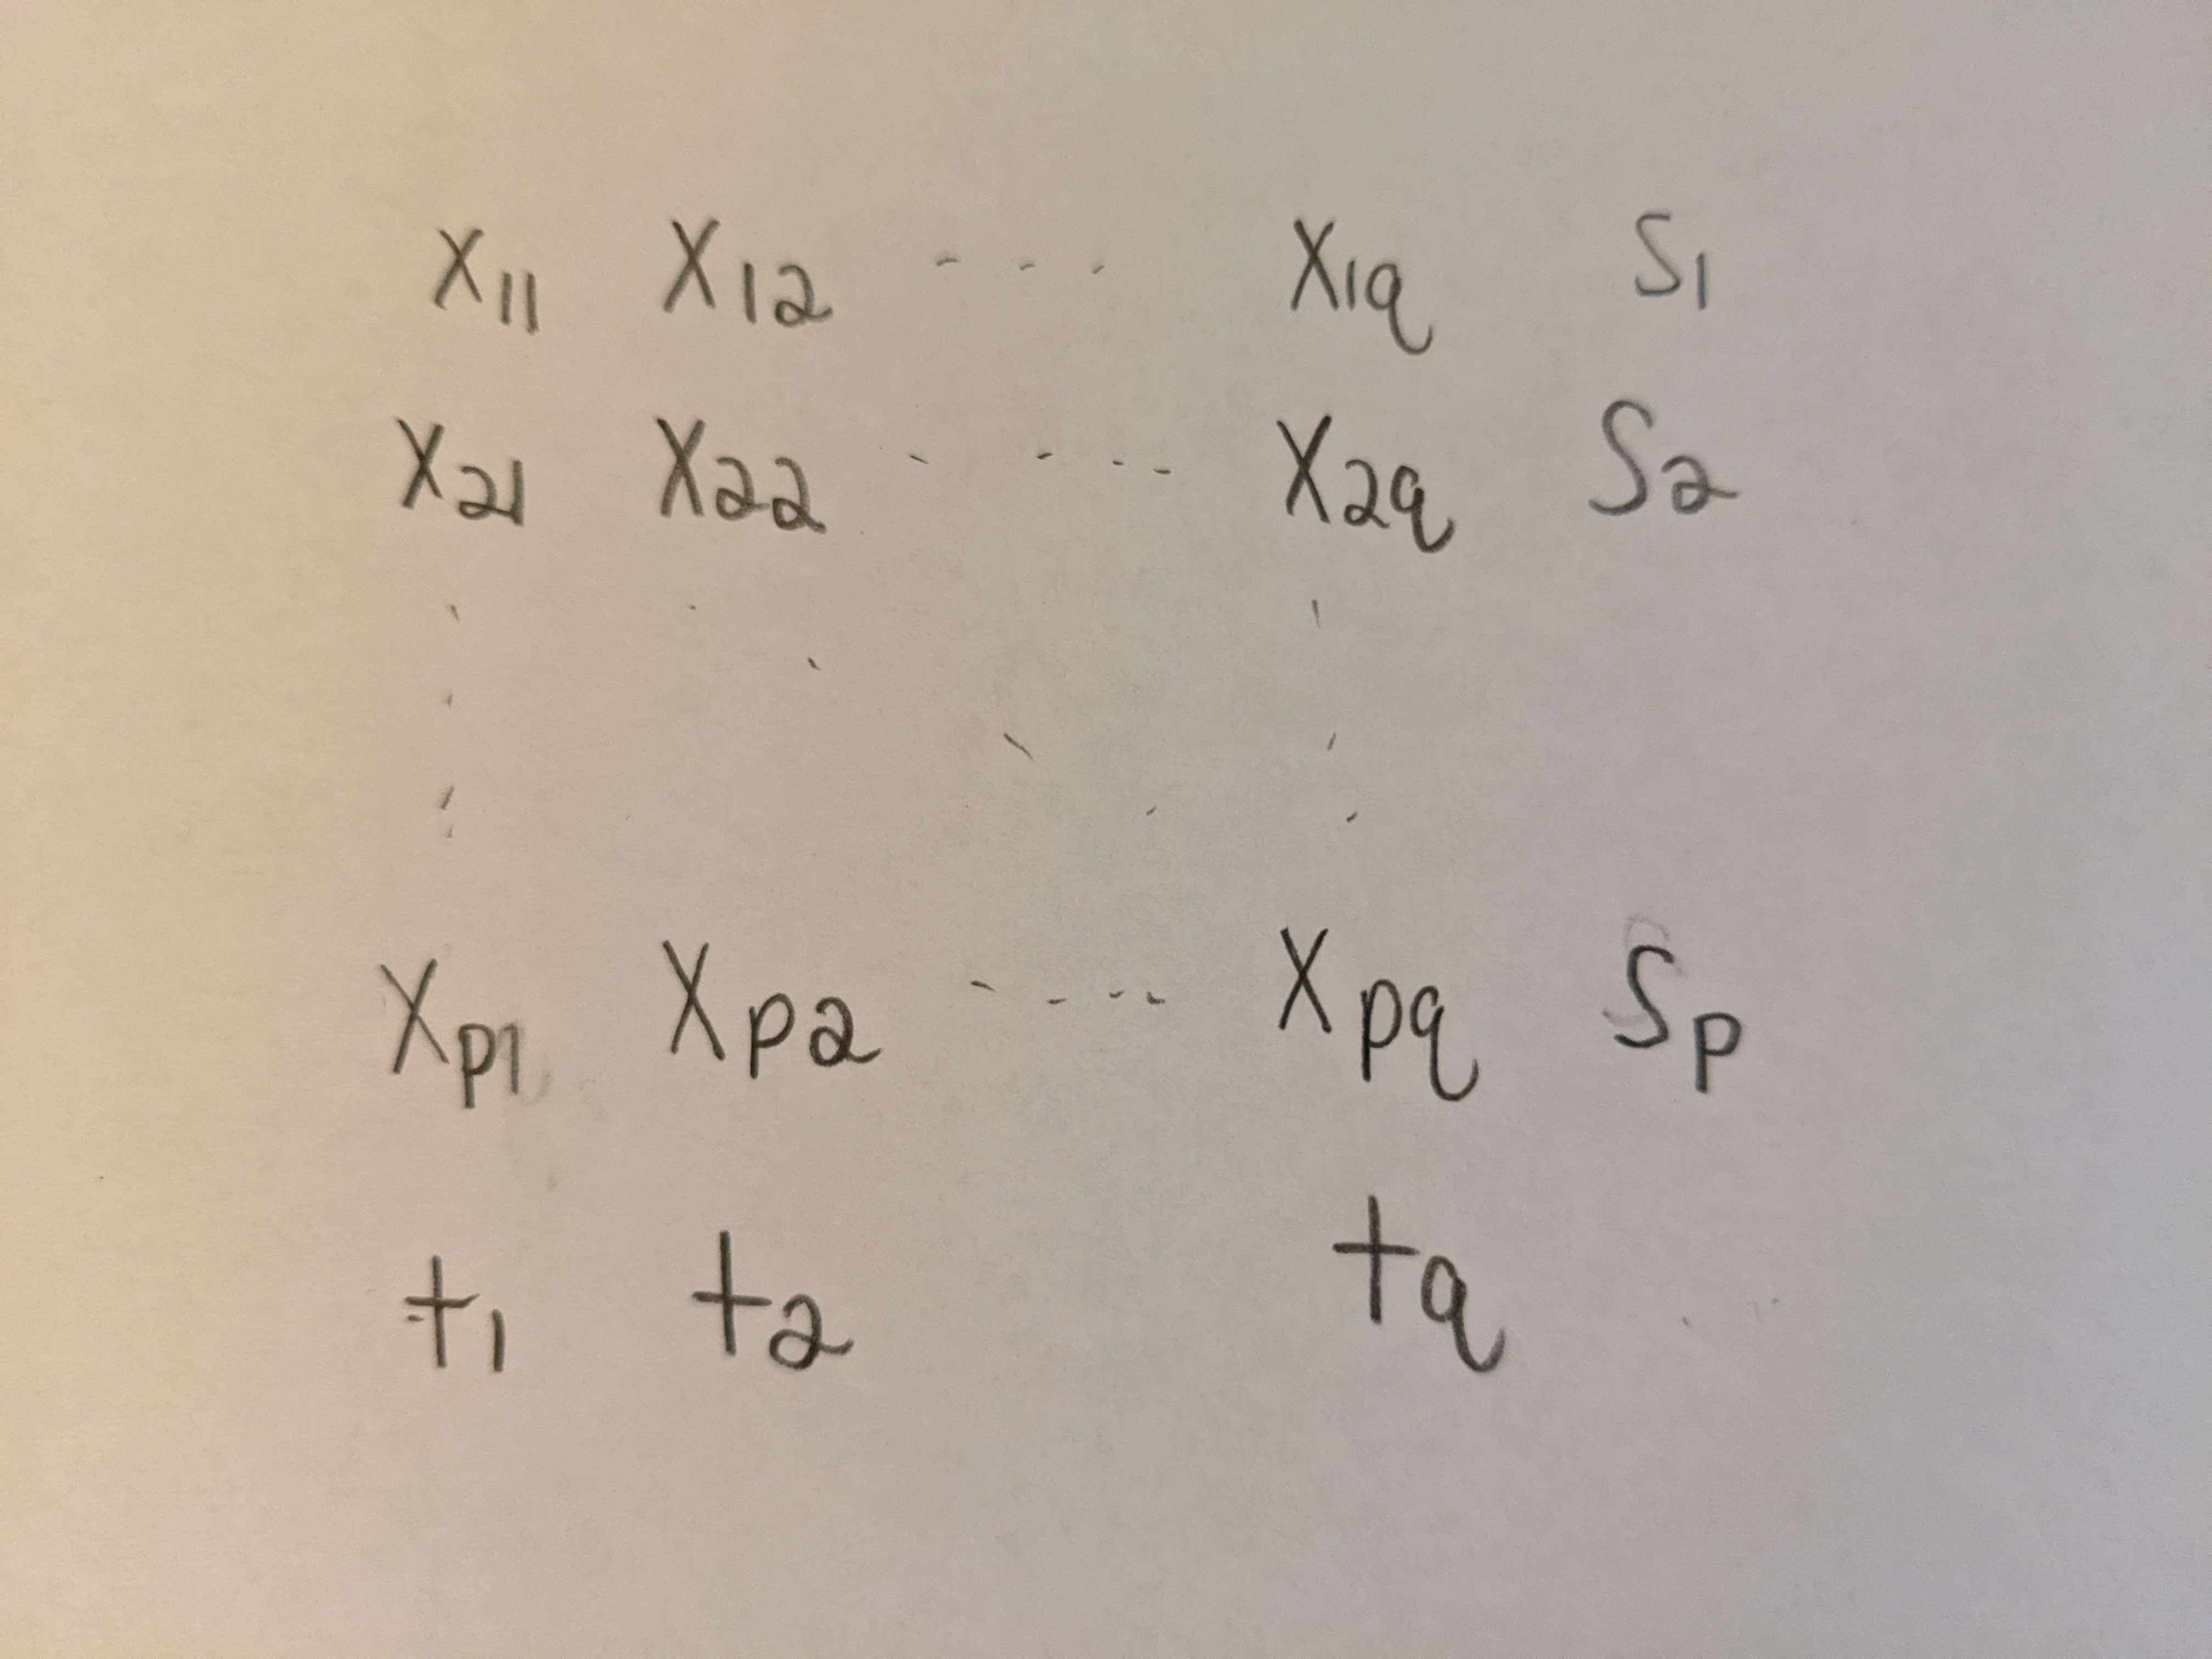
\includegraphics[width=\textwidth]{pic1}
%\end{figure}